\documentclass[11pt]{amsart}
\usepackage{geometry}                % See geometry.pdf to learn the layout options. There are lots.
\geometry{letterpaper}                   % ... or a4paper or a5paper or ... 
%\geometry{landscape}                % Activate for for rotated page geometry
%\usepackage[parfill]{parskip}    % Activate to begin paragraphs with an empty line rather than an indent
\usepackage{graphicx}
\usepackage{amssymb}
\usepackage{epstopdf}
\usepackage[usenames,dvipsnames]{color}
\usepackage{fancyvrb}
\usepackage{listings}
\usepackage{booktabs,footmisc}
\usepackage{hyperref}
\usepackage[all]{hypcap}

\usepackage{topcapt}


 
% include the lines below to use a nicer fixed-width font than the default one
 
\lstset{fancyvrb=true}
\lstset{
	basicstyle=\small\tt,
	identifierstyle=,
	commentstyle=\color{Bittersweet},
	stringstyle=\color{red},
	showstringspaces=false,
	tabsize=3,
	numbers=left,
	captionpos=b,
	xleftmargin=2em
%	numberstyle=\tiny
	%stepnumber=4
	}
\DeclareGraphicsRule{.tif}{png}{.png}{`convert #1 `dirname #1`/`basename #1 .tif`.png}

\title{Rebellion Model Description}
\author{Grace I. Lin - GSoC 2011}
%\date{\today}                                           % Activate to display a given date or no date

\begin{document} 
\maketitle

\tableofcontents 

\section{Model Description}

\begin{figure}[h!]
\centering
\vspace{.2in}
\centerline {
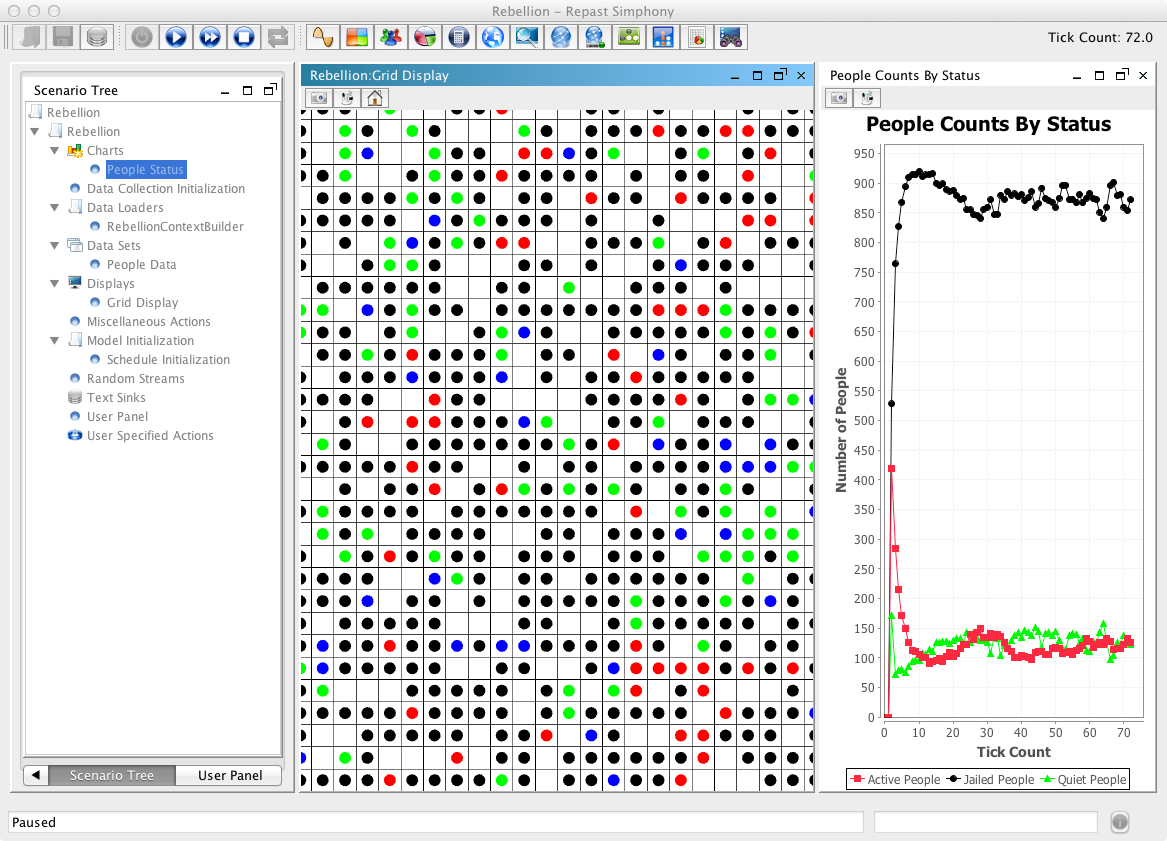
\includegraphics[width=6in]{Images/rebellion.png}}
\caption{Rebellion Model}
\label{fig:rebellion}
\end{figure}

The rebellion model (Figure \ref{fig:rebellion}) simulates how a group of people rebels against the authority (cops).  Each person is in one of the three states:
\begin{itemize}
\item \textbf{active}: red color; person decides to rebel (see calculation below for becoming an active person)
\item \textbf{jailed}: black color; active person arrested by cops; remain in jail until jail term expires
\item \textbf{quiet}: green color; neither active nor jailed
\end{itemize}

The cops (blue color) will randomly arrest active people within the visibility area.  To become an active (rebel), the person calculates his/her level of grievance and arrest probability:
\begin{itemize}
\item[] $ grievance = perceived\_hardship \times (1 - government\_legitimacy) $
\item[] $ arrest\_probability = 1-\exp \bigg ( -k \bigg \lfloor \frac{num\_of\_cops}{num\_of\_active\_people} \bigg \rfloor \bigg) $
\item[] $ \text{\emph{rebel  if} } (grievance - risk\_aversion \times arrest\_probability) > threshold $
\end{itemize}

where 
\begin{itemize}
\item[] \emph{perceived\_hardship} = 1.0 (fixed for lifetime) 
\item[] \emph{government\_legitimacy} = between 0 and 1; user specified 
\item[] \emph{k} = constant for one cop and one person within vision = 2.3 
\item[] \emph{risk\_aversion} = 1.0 (fixed for lifetime) 
\item[] \emph{threshold} = 0.1 
\end{itemize}

\section{Files and GUI}

Source files and description:
\begin{itemize}
\item[] src/rebellion/\textbf{Constants.java} : list of constants
\item[] src/rebellion/\textbf{Cop.java} : class for cop
\item[] src/rebellion/\textbf{CoverageCounter.java} : counts number of people in different states; used for data sets and charts in GUI Scenario Tree
\item[] src/rebellion/\textbf{Person.java} : class for person
\item[] src/rebellion/\textbf{RebellionContextBuilder.java} : set up environment initially
\item[] src/rebellion/\textbf{SMUtils.java} : miscellaneous functions
\item[] src/rebellion.observer/\textbf{PersonStyleOLG2D.java} : color assignment for cop/person
\end{itemize}

Remember to setup the grid and space projections in the resource folder "Rebellion.rs": in context node, add projection for type=continuous space and id=space, and add projection for type=grid and id=grid.  The id's can be found in the file Constants.java.  Once we run the Rebellion model, set up the Scenario Tree as follow:\\
\begin{itemize}
\item \textbf{Data Loaders} : Use RebellionContextBuilder
\item\textbf{Display}: Projection with grid, agents are Person and Cop, and agent style is  rebellion.observer.PersonStyleOLG2D for both Person and Cop
\item \textbf{Data Sets}: One for each active, quiet, and jailed people count from CoverageCounter.  Include a Title column for each data set so the chart will treat the counts in each data set as one series.  For example for active people, the Agent Class is CoverageCounter, agent mappings have column name Tick, ActivePeopleCount (source is getActivePeopleCount()), and Title (use Add $\rightarrow$ Add Using Wizards, and set value="Number of Active People")
\item \textbf{Charts}: One for each active, quiet, and jailed people data sets.  For example for active people count, X-Axis is Tick, Y-Axis Value is ActivePeopleCount with Series Name as Title.
\end{itemize}

\section{Model Parameters} 

\begin{figure}[h!]
\centering
\vspace{.2in}
\centerline {
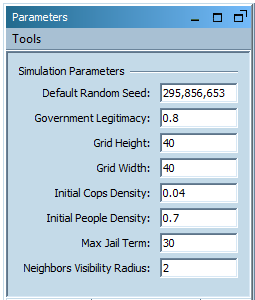
\includegraphics{Images/rebellion_param.png}}
\caption{Rebellion Model - Parameters}
\label{fig:param}
\end{figure}

User-specified parameters are shown in Figure \ref{fig:param} with descriptions as follow:

\begin{itemize}
\item \textbf{Government Legitimacy}:  Number of rows.
\item \textbf{Grid Height}:  Number of columns.
\item \textbf{Grid Width}:  Number of rows.
\item \textbf{Initial Cops Density}:  Percentage of grid size populated by cops.
\item \textbf{Initial People Density}:  Percentage of grid size populated by people.
\item \textbf{Max Jail Term}:  Maximum turns for people who are jailed.
\item \textbf{Neighbors Visibility Radius}:  Radius of area that the agent can see.
\end{itemize}
\vspace{.2in}


\section {References}

\begin{itemize}
\item NetLogo's termites model: \emph{http://ccl.northwestern.edu/netlogo/models/Rebellion}
\item Modeling civil violence: An agent-based computational approach (\emph{http://www.pnas.org/content/99/suppl.3/7243.full})
\end{itemize}

\end{document}  